\ifSTANDALONE
\section{Konzept}
\fi
\ifEMBED
\subsection{Konzept}
\fi

Das Stellen eines fremderregten Gleichstrommotors erfolgt über die
angelegte Ankerspannung. Eine variable Ankerspannung kann mittels einer 
zeitlichen Mittelung der anliegenden Spannung realisert werden. Somit
ist es möglich eine fremderregte Gleichstrommaschine mittels einer
konstanten Gleichspannung einzustellen. Die Mittelung der Ankerspannung
bildet die Basis des vorliegenden Konzepts für den DC-Motor-Treiber.

\ifSTANDALONE
\subsection{Annahmen und Abschätzungen}\label{sec:annahmen}
\fi
\ifEMBED
\subsubsection{Annahmen und Abschätzungen}\label{sec:annahmen}
\fi
Für das vorliegende Konzept gilt die Annahme, dass das Erregerfeld mittels
Permanentmagneten realisiert und das Erregerfeld konstant ist. Diese
Annahme ist gewählt, da fremderregte Gleichstrommaschinen ohne
Permanentmagneten einen Erregerstrom benötigen, welcher das Erregerfeld
erzeugt. Im einfachsten Fall ist dies eine Konstantstromquelle. Eine solche
Maschine benötigt mehr elektrische Energie und erfordert zusätzlichen
Hardwareaufwand.

\noindent Die Drehzahl einer idealen fremderregten Gleichstrommaschine mit 
konstantem Erregerfeld korreliert mit dem Faktor $-1$ zum Strom. Der Strom 
einer solchen Maschine korreliert wiederum mit der Belastung 
\cite[p.163]{smps}. Dieses Verhalten zwischen Belastung und Drehzahl ist in 
Abbildung \ref{fig:ideal-dc-curve} dargestellt.

\begin{figure}[h!]
    \centering
    \begin{tikzpicture}
        % Achsen
        \draw[->] (-0.5,0) -- (8,0) node[anchor=north] {$I, M$};
        \draw[->] (0,-0.5) -- (0,4) node[anchor=east] {$\omega_m$};
        % Klemmenspannung
        \draw[blue, thick] (0,3) -- (7,3) node[anchor=west] {$U_K$};
        % induzierte Spannung
        \draw[red, thick] 
            (0,3) node[anchor=east] {$\omega_0$} -- 
            (7,0) node[midway, above right] {$\omega \sim U_i$};
        
    \end{tikzpicture}
    \caption{Winkelgeschwindigkeit einer idealen fremderregten 
        Gleichstrommaschine}
    \label{fig:ideal-dc-curve}
\end{figure}

\ifSTANDALONE
\subsection{Ziel}
\fi
\ifEMBED
\subsubsection{Ziel}
\fi
Es ist eine Hardware zu entwicklen, welche es ermöglicht, die
Winkelgeschwindigkeit einer fremderregten Gleichstrommaschine mit
Permanentmagneten zu regeln.

\ifSTANDALONE
\subsection{Funktionsweise}
\fi
\ifEMBED
\subsubsection{Funktionsweise}
\fi
Um die Klemmenspannung der Gleichstrommaschine zu stellen, wird eine
H-Brücke verwendet. Diese kann je nach Bedarf individuell ausgelegt
werden. Die Ansteuerung der H-Brücke erfolgt mittels des Treiberchips
A3941 von Allegro Microsystems. Das Interface, welches der
Treiberchip zur Verfügung stellt, wird mittels eines Mikrocontrollers
bedient, welcher ebenfalls individuell gewählt ist.

\begin{figure}[h!]
    \centering
    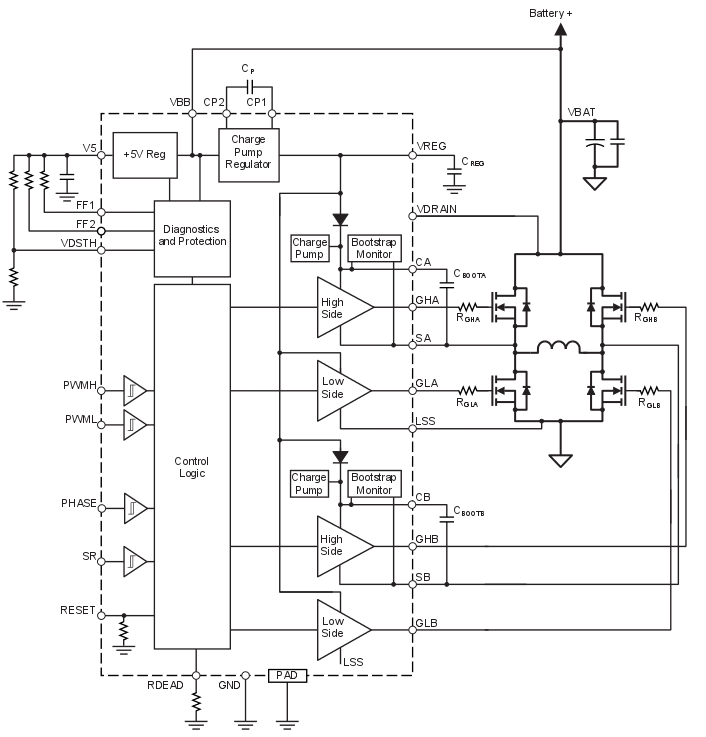
\includegraphics[width=0.75\textwidth]{\DCPath/fig/a3941-functional.png}
    \caption[Blockschaltbild des A3941]{Blockschaltbild des A3941 \cite{Datasheet:A3941}}
    \label{fig:a3941-functional}
\end{figure}

\noindent Die Regelung der Winkelgeschwindigkeit eines angeschlossenen Motors 
kann mit verschiedenen Ansätzen realisiert werden. Gemeinsam ist dabei stets die
Stellgrösse, welche durch das PWM Signal gegeben ist, als auch die
Winkelgeschwindigkeit der Maschine, welche die Regelgrösse darstellt.

\noindent Die Regelung muss auf einem Feedback der Winkelgeschwindigkeit 
basieren. Wird von einer idealen Maschine ausgegangen, muss dieses Feedback 
nicht zwingend durch einen Encoder generiert werden, sondern kann implizit 
durch den Strom gegeben sein, wie in Abbildung \ref{fig:ideal-dc-curve} 
dargestellt. Mit den getroffenen Annahmen aus Abschnitt \ref{sec:annahmen} 
kann somit auf ein explizites Feedback der Winkelgeschwindigkeit verzichtet 
werden. 

\ifSTANDALONE
\subsection{Regelung}
\fi
\ifEMBED
\subsubsection{Regelung}
\fi
Für die Ansteuerung der H-Brücke bzw. des Treiberchips A3941 wird ein PWM
Signal benötigt. Dieses kann in Hardware auf dem Treiberboard implementiert
werden, mittels eines Sägezahngenerators und einem Komparator. Der zweite
Komparatoreingang wird dazu an das Feedback des Stromes angeschlossen, was
ein zur Winkelgeschwindigkeit angepasstes PWM Signal generiert.

\noindent Alternativ zu dieser Regelung kann das Feedback des Stromes auch zu 
einem Mikrocontroller geführt werden, welcher dieses auswertet und ein passendes
PWM Signal generiert.

\begin{figure}[h!]
    \centering
    \begin{subfigure}[b]{0.45\textwidth}
        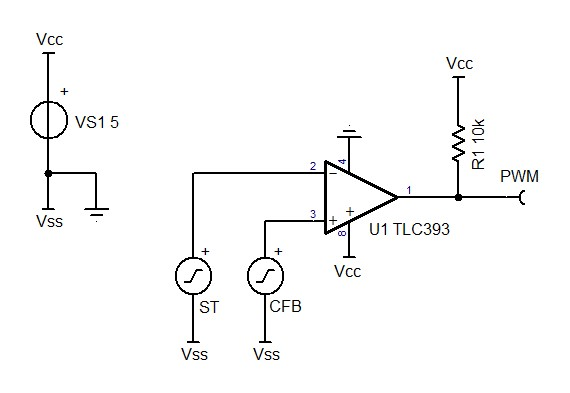
\includegraphics[width=\textwidth]{\DCPath/sim/sch-pwm-01.jpg}
        \caption{Prinzipschema mit dem Komparator TLC393}
    \end{subfigure}
    \begin{subfigure}[b]{0.45\textwidth}
        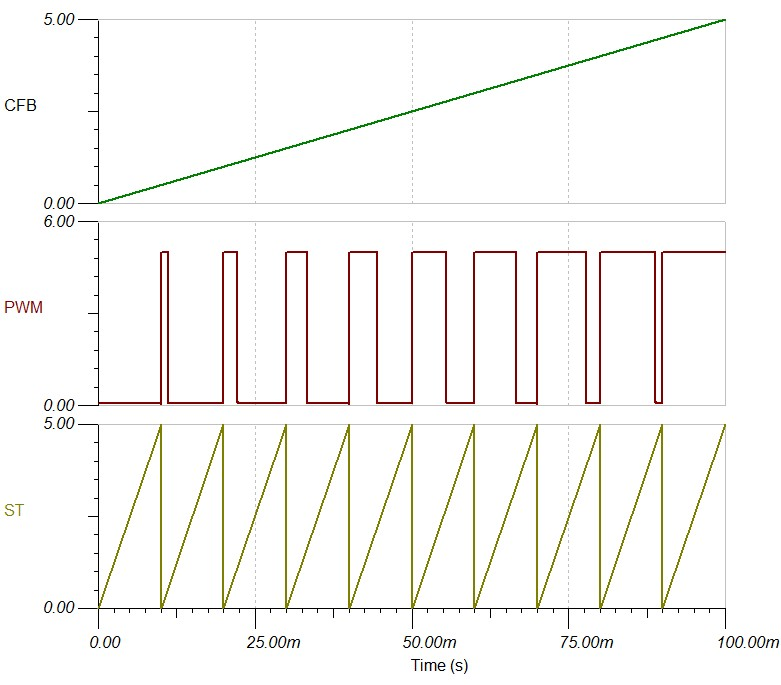
\includegraphics[width=\textwidth]{\DCPath/sim/pwm-01.jpg}
        \caption{Simulationsergebnisse für lineares Feedback}
    \end{subfigure}
    \caption{Simulation eines PWM-Generator mit Komparator}
\end{figure}

\begin{figure}[h!]
    \centering
    \begin{subfigure}[b]{0.45\textwidth}
        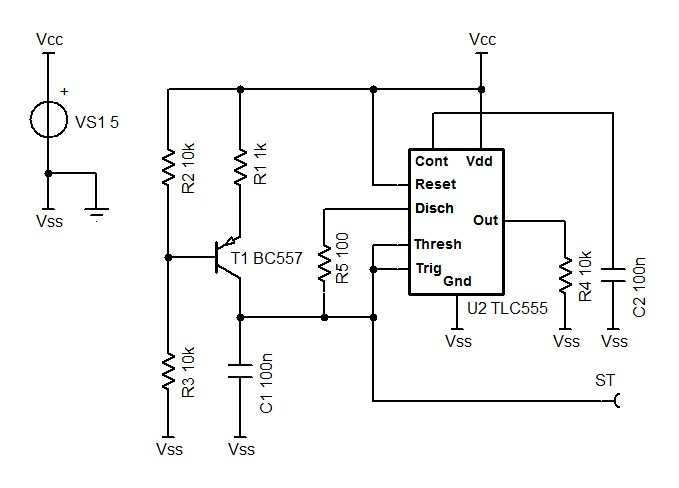
\includegraphics[width=\textwidth]{\DCPath/sim/sch-sawtooth-01.jpg}
        \caption{Sägezahntgenerator mit Timer TLC555}
    \end{subfigure}
    \begin{subfigure}[b]{0.45\textwidth}
        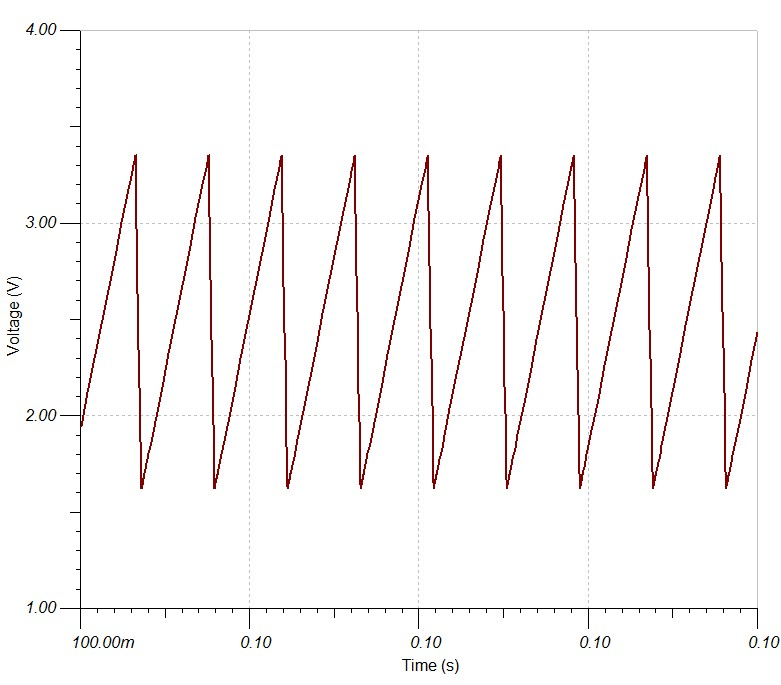
\includegraphics[width=\textwidth]{\DCPath/sim/sawtooth-01.jpg}
        \caption{Simulationsergebnisse ($f_{ST} \approx 9.3$kHz)}
    \end{subfigure}
    \caption{Simulation eines Sägezahngenerators}
    \label{fig:sawtooth}
\end{figure}

\noindent Ein passender Baustein zur Erzeugung ist der Timer TLC555, wie in der
Abbildung \ref{fig:sawtooth} dargestellt. Das Feedback des Stromes kann
dabei auf verschiedene Weisen implementiert werden. Einerseits gibt es eine
kostengünstige Variante mittels dem Einsatz eines Shunt-Widerstands. Dieser
bietet im Idealfall ein lineares Varhalten. In der Realität führt der
Einfluss der Temperatur zu einer deutlichen Nichtlinearität dieses
Messmittels. Eine Alternative zum Shunt-Widerstands bietet der Einsatz von
Hall-Effekt-Stromwandlern, welche den Strom linearisiert als Spannungssignal
ausgeben. Ein solcher Baustein ist der ACS712 der Allegro Microsystems,
welcher im SMD Format verfügbar ist, bis zu einem Strom von 30A.

\noindent Ist eine genaue Drehzahl nicht von Bedeutung, kann auf die Regelung der
Winkelgeschwindigkeit verzichtet werden. Dies gilt insbesondere, wenn eine
hohe Übersetzung vorliegt, welche verhindert, dass die Winkelgeschwindigkeit
der Gleichstrommaschine einbricht, bei entsprechender Belastung. Für diesen
Fall kann das PWM fix eingestellt werden und lediglich mit einem Enable
Signal gearbeitet werden. Dies lässt sich mit einer logischen AND Funktion
realisieren für das PWM Signal. Eine mögliche Implementierung ist in der
Abbildung \ref{fig:and} dargestellt.

\begin{figure}[h!]
    \centering
    \begin{subfigure}[b]{0.45\textwidth}
        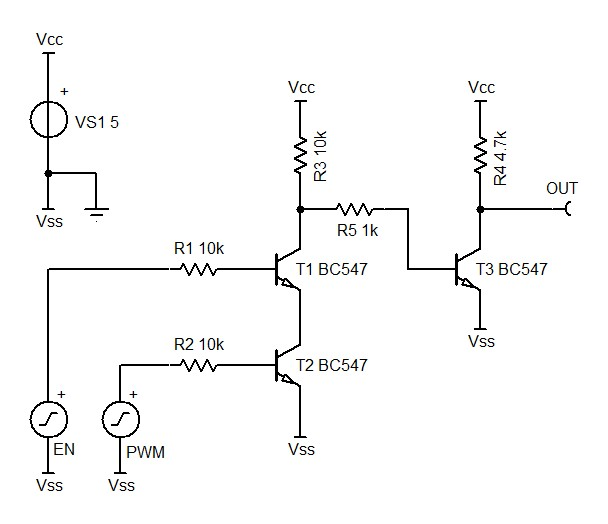
\includegraphics[width=\textwidth]{\DCPath/sim/sch-and-01.jpg}
        \caption{AND-Schaltung mit NPN-Transistoren}
    \end{subfigure}
    \begin{subfigure}[b]{0.45\textwidth}
        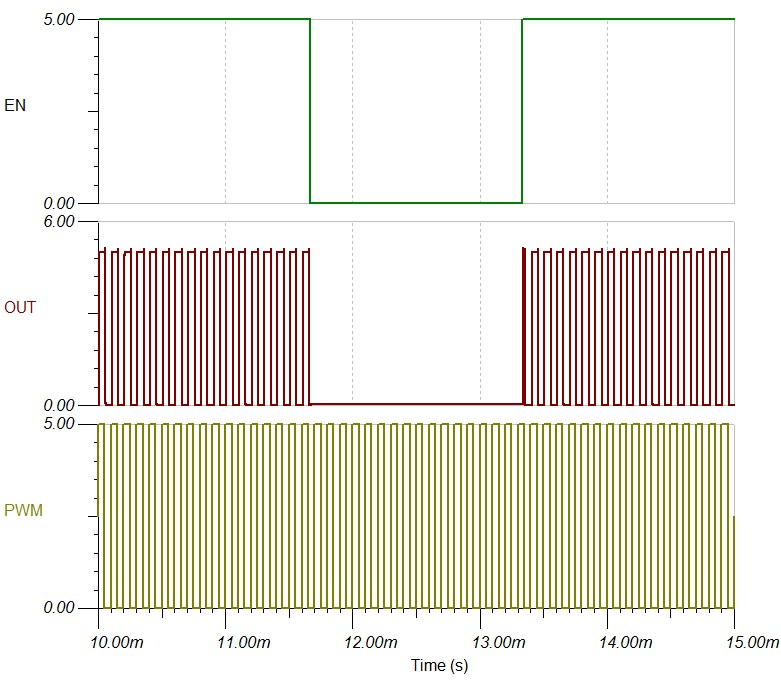
\includegraphics[width=\textwidth]{\DCPath/sim/and-01.jpg}
        \caption{Simulationsergebnisse}
    \end{subfigure}
    \caption{Simulation einer AND-Schaltung realisiert mit
        Bipolartransistoren}
    \label{fig:and}
\end{figure}

